% !TeX program = xelatex
\documentclass[a4paper,10pt]{article}

% ============================================================================
% កញ្ចប់បណ្ណាល័យ (Packages) – តាមលំនាំ NGS Preah Krasang (ls_plan.tex)
% បរិបទ៖ គ្មានស្លាយ LCD និងគ្មានម៉ាស៊ីនគិតលេខ — ប្រើសន្លឹកកិច្ចការសិស្ស (ស-ខ្មៅ) និងក្ដារខៀនជាគោល
% ============================================================================
\usepackage[a4paper, left=0.95cm, right=0.95cm, top=0.85cm, bottom=0.92cm, footskip=0.52cm]{geometry}
\usepackage{amsmath}
\usepackage{unicode-math}
\usepackage{fontspec}
\usepackage{array, longtable, multirow, colortbl}
\usepackage[table]{xcolor}
\usepackage{enumitem}
\usepackage{pifont}
\usepackage{fancyhdr}
\usepackage{tikz}
\usetikzlibrary{calc, arrows.meta, angles, quotes, decorations.markings, decorations.pathreplacing, patterns, babel}

\makeatletter
\let\@expl@@@mark@update@singlecol@structures@@\relax
\makeatother

\providecommand{\NGSFindFonts}{%
  \IfFileExists{C:/Windows/Fonts/cambria.ttc}{%
    \def\NGSSysPath{C:/Windows/Fonts/}%
    \def\NGSUserPath{C:/Users/KIT/AppData/Local/Microsoft/Windows/Fonts/}%
  }{%
    \IfFileExists{./fonts/KhmerOSsiemreap.ttf}{\def\NGSSysPath{./fonts/}\def\NGSUserPath{./fonts/}}{%
    \IfFileExists{../fonts/KhmerOSsiemreap.ttf}{\def\NGSSysPath{../fonts/}\def\NGSUserPath{../fonts/}}{%
    \IfFileExists{../../fonts/KhmerOSsiemreap.ttf}{\def\NGSSysPath{../../fonts/}\def\NGSUserPath{../../fonts/}}{%
    \IfFileExists{../../../fonts/KhmerOSsiemreap.ttf}{\def\NGSSysPath{../../../fonts/}\def\NGSUserPath{../../../fonts/}}{%
    \IfFileExists{../../../../fonts/KhmerOSsiemreap.ttf}{\def\NGSSysPath{../../../../fonts/}\def\NGSUserPath{../../../../fonts/}}{%
    \IfFileExists{../../../../../fonts/KhmerOSsiemreap.ttf}{\def\NGSSysPath{../../../../../fonts/}\def\NGSUserPath{../../../../../fonts/}}{%
    \IfFileExists{../../../../../../fonts/KhmerOSsiemreap.ttf}{\def\NGSSysPath{../../../../../../fonts/}\def\NGSUserPath{../../../../../../fonts/}}{%
      \def\NGSSysPath{../../../../../../../fonts/}\def\NGSUserPath{../../../../../../../fonts/}%
    }}}}}}}%
  }%
}
\NGSFindFonts

\setmathfont[Path={\NGSSysPath}, FontIndex=1, Scale=1.02]{cambria.ttc}
\defaultfontfeatures{Ligatures=TeX}

\setmainfont[
  Path={\NGSUserPath}, Extension=.ttf, Script=Khmer,
  BoldFont={KhmerOSsiemreap}, BoldFeatures={FakeBold=1.8},
  ItalicFont={KhmerOSsiemreap}, ItalicFeatures={FakeSlant=0.25},
  BoldItalicFont={KhmerOSsiemreap}, BoldItalicFeatures={FakeBold=1.8, FakeSlant=0.25}
]{KhmerOSsiemreap}

\newfontfamily\muol[Path={\NGSUserPath}, Extension=.ttf, Script=Khmer]{KhmerOSmuollight}
\newfontfamily\TimesEn[Path={\NGSSysPath}, Extension=.ttf, Scale=1.00, BoldFont={timesbd}, ItalicFont={timesi}, BoldItalicFont={timesbi}]{times}
\newfontfamily\NagaBold[Path={\NGSUserPath}, Extension=.ttf]{AKbalthom Naga Bold}
\newfontfamily\CalibriFont[Path={\NGSSysPath}, Extension=.ttf]{calibri}
\newfontfamily\Tacteing[Path={\NGSUserPath}]{TACTENG.TTF}
\newfontfamily\CourierBullet[Path={\NGSSysPath}, Extension=.ttf]{cour}
\newcommand{\wcirc}{{\CourierBullet\fontsize{9.5pt}{11pt}\selectfont o}}

\XeTeXlinebreaklocale "km"
\XeTeXlinebreakskip = 0pt plus 1pt minus 0.1pt

\definecolor{stepgray}{HTML}{D9D9D9}
\definecolor{headgray}{HTML}{F2F2F2}
\definecolor{boxgray}{HTML}{D9D9D9}
\definecolor{darkred}{HTML}{C00000}
\definecolor{red5e}{HTML}{FF0000}

\pagestyle{fancy}
\fancyhf{}
\renewcommand{\headrulewidth}{0pt}
\fancyfoot[R]{\CalibriFont\fontsize{11pt}{13pt}\selectfont\thepage}

\setlength{\parindent}{0pt}
\setlength{\parskip}{0pt}
\setlength{\tabcolsep}{3.8pt}

\newcolumntype{L}[1]{>{\raggedright\arraybackslash}p{#1}}
\newcolumntype{C}[1]{>{\centering\arraybackslash}p{#1}}

\newcommand{\en}[1]{{\TimesEn #1}}
\newcommand{\enbf}[1]{{\TimesEn\textbf{#1}}}
\newcommand{\unit}[1]{\,\text{\en{#1}}}
\newcommand{\fiveE}[1]{{\NagaBold\fontsize{9.5pt}{13pt}\selectfont\textcolor{red5e}{#1}}}
\newcommand{\timenote}[1]{\textcolor{darkred}{\textit{#1}}}
\newcommand{\redsub}[1]{\textcolor{darkred}{#1}}
\newcommand{\graybox}[1]{\colorbox{boxgray}{\strut\hspace{2pt}#1\hspace{2pt}}}
\newcommand{\ditem}{\tikz[baseline=-0.5ex]\fill (0,0.42ex) -- (0.42ex,0) -- (0,-0.42ex) -- (-0.42ex,0) -- cycle;\hspace{0.3em}}
\newcommand{\cnum}[1]{{\fontsize{10.5pt}{12pt}\selectfont\ding{\numexpr181+#1\relax}}\hspace{0.15em}}
\newcommand{\cfig}[1]{\par\vspace{3pt}{\centering #1\par}\vspace{3pt}}
\newcommand{\stepheader}[1]{\multicolumn{3}{|c|}{\cellcolor{stepgray}\muol #1} \\* \noalign{\hrule height 0.4pt}}
\newcommand{\khmflourish}{{\Tacteing\fontsize{36pt}{14pt}\selectfont\raisebox{-5pt}{3}}}

% ============================================================================
% ម៉ាក្រូគូសរូប TikZ ស-ខ្មៅ ១០០% សម្រាប់មេរៀន ២.៤.៦ (ក និង ខ) ឫសការេ និងឫសគូប (ROOT1)
% ============================================================================

% ១. E1 Engage: អន្ទាក់សញ្ញា \sqrt{16} ទល់នឹង x^2=16 និង \sqrt{-9} ទល់នឹង \sqrt[3]{-8}
\newcommand{\figEngageROOTA}{%
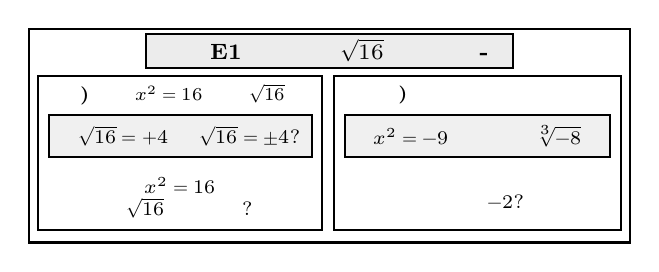
\begin{tikzpicture}[x=0.96cm, y=0.92cm, every node/.style={font=\scriptsize, text=black}]
  \draw[black, line width=0.95pt] (0,0) rectangle (7.95,2.95);
  \node[fill=gray!15, draw=black, line width=0.6pt, inner sep=2pt, font=\footnotesize\bfseries] at (3.975,2.65) {បេសកកម្ម \en{E1}៖ អន្ទាក់សញ្ញា $\sqrt{16}$ និងច្រកសញ្ញាគូ-សេស};

  \draw[black, line width=0.8pt] (0.12,0.18) rectangle (3.88,2.30);
  \node[font=\fontsize{6.6pt}{8.5pt}\selectfont\bfseries] at (2.00,2.04) {១) សមីការ $x^2 = 16$ ទល់នឹង $\sqrt{16}$};
  \draw[black, line width=0.75pt, fill=gray!12] (0.26,1.18) rectangle (3.74,1.76);
  \node at (2.00,1.47) {តើ $\sqrt{16} = +4$ \;ឬ\; $\sqrt{16} = \pm 4$?};
  \node[align=center] at (2.00,0.62) {ហេតុអ្វី $x^2=16$ មានឫសពីរ\\តែ $\sqrt{16}$ មានតម្លៃតែមួយ?};

  \draw[black, line width=0.8pt] (4.04,0.18) rectangle (7.83,2.30);
  \node[font=\fontsize{6.5pt}{8.5pt}\selectfont\bfseries] at (5.935,2.04) {២) ឫសការេ ទល់នឹង ឫសគូបអវិជ្ជមាន};
  \draw[black, line width=0.75pt, fill=gray!12] (4.18,1.18) rectangle (7.69,1.76);
  \node at (5.935,1.47) {$x^2 = -9$ \quad ទល់នឹង \quad $\sqrt[3]{-8}$};
  \node[align=center] at (5.935,0.62) {តើមួយណា\textbf{គ្មានឫស} ហើយមួយណា\\មានឫសស្មើ $-2$?};
\end{tikzpicture}}

% ២. E2 POE 1 & 2: តារាងទ្វេទិស សមីការ ទល់នឹង រ៉ាឌីកាល់ និងច្រកសញ្ញាគូ-សេស
\newcommand{\figDualTrackROOTA}{%
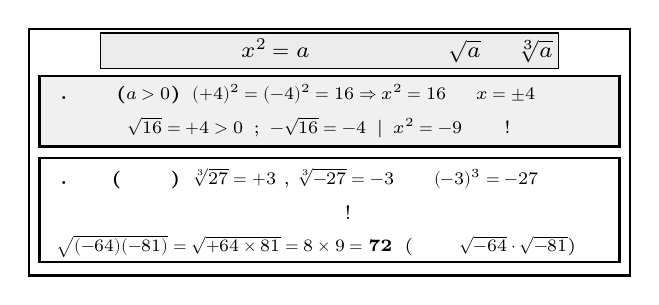
\begin{tikzpicture}[x=0.96cm, y=0.92cm, every node/.style={font=\scriptsize, text=black}]
  \draw[black, line width=0.95pt] (0,0) rectangle (7.95,3.40);
  \node[fill=gray!15, draw=black, line width=0.6pt, inner sep=2pt, font=\footnotesize\bfseries] at (3.975,3.10) {តារាងទ្វេទិស៖ សមីការ $x^2=a$ ទល់នឹង និមិត្តសញ្ញា $\sqrt{a}$ និង $\sqrt[3]{a}$};

  % Top box: Square roots
  \draw[black, line width=0.85pt, fill=gray!12] (0.14,1.78) rectangle (7.81,2.75);
  \node[anchor=west, font=\fontsize{6.4pt}{8pt}\selectfont] at (0.22,2.50) {\textbf{ក. ឫសការេ ($a>0$)៖} $(+4)^2 = (-4)^2 = 16 \Rightarrow x^2=16$ មាន $x = \pm 4$};
  \node[anchor=west, font=\fontsize{6.4pt}{8pt}\selectfont] at (0.22,2.04) {\textbf{និមិត្តសញ្ញា៖} $\sqrt{16} = +4 > 0$ \,;\, $-\sqrt{16} = -4$ \,\textbar\, $x^2=-9$ \textbf{គ្មានឫស}!};

  % Bottom box: Cube roots & Product sign gate
  \draw[black, line width=0.85pt] (0.14,0.18) rectangle (7.81,1.62);
  \node[anchor=west, font=\fontsize{6.4pt}{8pt}\selectfont] at (0.22,1.34) {\textbf{ខ. ឫសគូប (រក្សាសញ្ញា)៖} $\sqrt[3]{27} = +3$ , $\sqrt[3]{-27} = -3$ ព្រោះ $(-3)^3 = -27$};
  \node[anchor=west] at (0.22,0.86) {\textbf{គន្លឹះផលគុណក្រោមរ៉ាឌីកាល់៖} គិតសញ្ញាក្នុងរ៉ាឌីកង់ជាមុន!};
  \node[anchor=west, font=\fontsize{6.3pt}{8pt}\selectfont] at (0.24,0.40) {$\sqrt{(-64)(-81)} = \sqrt{+64\times 81} = 8\times 9 = \mathbf{72}$ \;(ហាមបំបែក $\sqrt{-64}\cdot\sqrt{-81}$)};
\end{tikzpicture}}

% ៣. E4 Geometric Square & Cube (គំរូ ២ ទំ.២៣)
\newcommand{\figGeomROOTA}{%
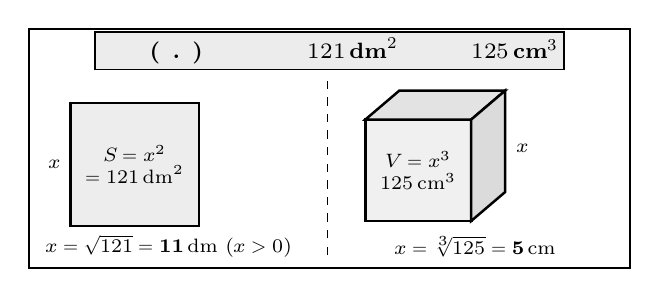
\begin{tikzpicture}[x=0.96cm, y=0.92cm, every node/.style={font=\scriptsize, text=black}]
  \draw[black, line width=0.95pt] (0,0) rectangle (7.95,3.30);
  \node[fill=gray!15, draw=black, line width=0.6pt, inner sep=2pt, font=\footnotesize\bfseries] at (3.975,3.00) {គំរូ ២ (ទំ.២៣)៖ ការេក្រឡាផ្ទៃ $121\unit{dm}^2$ និងគូបមាឌ $125\unit{cm}^3$};

  % Left: Square
  \draw[black, line width=0.95pt, fill=gray!14] (0.55,0.58) rectangle (2.25,2.28);
  \node[align=center] at (1.40,1.43) {$S = x^2$\\$= 121\unit{dm}^2$};
  \node at (1.85,0.30) {$x = \sqrt{121} = \mathbf{11\unit{dm}}$ ($x>0$)};
  \node[left] at (0.55,1.43) {$x$};

  \draw[black, dashed, line width=0.6pt] (3.95,0.18) -- (3.95,2.68);

  % Right: 3D Cube
  \draw[black, line width=0.95pt, fill=gray!12] (4.45,0.65) rectangle (5.85,2.05);
  \draw[black, line width=0.9pt, fill=gray!22] (4.45,2.05) -- (4.90,2.45) -- (6.30,2.45) -- (5.85,2.05) -- cycle;
  \draw[black, line width=0.9pt, fill=gray!28] (5.85,0.65) -- (6.30,1.05) -- (6.30,2.45) -- (5.85,2.05) -- cycle;
  \node[align=center] at (5.15,1.35) {$V = x^3$\\$125\unit{cm}^3$};
  \node[right] at (6.32,1.65) {$x$};
  \node at (5.90,0.30) {$x = \sqrt[3]{125} = \mathbf{5\unit{cm}}$};
\end{tikzpicture}}

% ៤. E5 Diagnostic Options A-D
\newcommand{\figExitCardsROOTA}{%
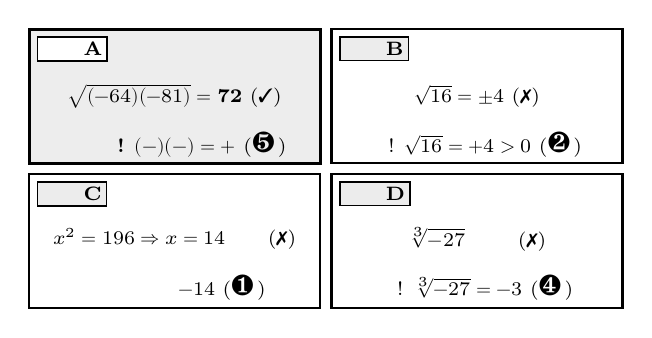
\begin{tikzpicture}[x=0.96cm, y=0.92cm, every node/.style={font=\scriptsize, text=black}]
  \draw[black, line width=1.1pt, fill=gray!14] (0,2.00) rectangle (3.85,3.85);
  \node[anchor=north west, fill=white, draw=black, line width=0.6pt, inner sep=1.8pt] at (0.10,3.75) {\textbf{ជម្រើស \en{A}}};
  \node at (1.925,2.92) {$\sqrt{(-64)(-81)} = \mathbf{72}$ (\ding{51})};
  \node at (1.925,2.25) {\textbf{ត្រឹមត្រូវ!} $(-)(-)=+$ (\cnum{5})};

  \draw[black, line width=0.9pt] (4.00,2.00) rectangle (7.85,3.85);
  \node[anchor=north west, fill=gray!15, draw=black, line width=0.6pt, inner sep=1.8pt] at (4.10,3.75) {\textbf{ជម្រើស \en{B}}};
  \node at (5.925,2.92) {$\sqrt{16} = \pm 4$ (\ding{55})};
  \node at (5.925,2.25) {ខុស! $\sqrt{16}=+4>0$ (\cnum{2})};

  \draw[black, line width=0.9pt] (0,0) rectangle (3.85,1.85);
  \node[anchor=north west, fill=gray!15, draw=black, line width=0.6pt, inner sep=1.8pt] at (0.10,1.75) {\textbf{ជម្រើស \en{C}}};
  \node at (1.925,0.95) {$x^2 = 196 \Rightarrow x = 14$ តែមួយ (\ding{55})};
  \node at (1.925,0.28) {ភ្លេចឫសអវិជ្ជមាន $-14$ (\cnum{1})};

  \draw[black, line width=0.9pt] (4.00,0) rectangle (7.85,1.85);
  \node[anchor=north west, fill=gray!15, draw=black, line width=0.6pt, inner sep=1.8pt] at (4.10,1.75) {\textbf{ជម្រើស \en{D}}};
  \node at (5.925,0.95) {$\sqrt[3]{-27}$ គ្មានឫស (\ding{55})};
  \node at (5.925,0.28) {ខុស! $\sqrt[3]{-27}=-3$ (\cnum{4})};
\end{tikzpicture}}

\begin{document}
\fontsize{10pt}{15.2pt}\selectfont

% -------------------- ក្បាលកិច្ចតែងការ --------------------
\begin{center}
  {\muol\fontsize{11pt}{16pt}\selectfont ព្រះរាជាណាចក្រកម្ពុជា}\\[2pt]
  {\muol\fontsize{10pt}{15pt}\selectfont ជាតិ សាសនា ព្រះមហាក្សត្រ}\\[1pt]
  \khmflourish
\end{center}

\vspace{-24pt}
{\muol\fontsize{9.5pt}{12.5pt}\selectfont
មន្ទីរអប់រំ យុវជន និងកីឡា ខេត្តកំពង់ធំ\\
ការិយាល័យអប់រំ យុវជន និងកីឡា ស្រុកកំពង់ស្វាយ\\
អនុវិទ្យាល័យព្រះក្រសាំង}

\vspace{1pt}
\begin{center}
  {\muol\fontsize{10pt}{14pt}\selectfont កិច្ចតែងការបង្រៀន}
\end{center}
\vspace{0pt}

% -------------------- ព័ត៌មានទូទៅ --------------------
{\renewcommand{\arraystretch}{0.98}
\hspace*{3.1cm}%
\begin{tabular}{@{}l l L{11.0cm}@{}}
  - \hspace{0.35cm} មុខវិជ្ជា & : & គណិតវិទ្យា ថ្នាក់ទី៨ (ពីជគណិត) \\
  - \hspace{0.35cm} ចំណងជើងមេរៀន & : & មេរៀនទី២៖ ស្វ័យគុណ \\
  - \hspace{0.35cm} ចំណងជើងរង & : & ៤.៦. ឫសការេ និងឫសគូបនៃចំនួនសនិទាន — ក និង ខ (ទំ.២២–២៤ និងលំហាត់ \#12–\#15 ទំ.២៦) \\
  - \hspace{0.35cm} រយៈពេល & : & ១ ម៉ោងសិក្សា (៥០ នាទី) \\
  - \hspace{0.35cm} បង្រៀនដោយ & : & ហុក ប៊ុនថែន \\
  - \hspace{0.35cm} កាលបរិច្ឆេទ & : & ថ្ងៃព្រហស្បតិ៍ ទី១៩ ខែវិច្ឆិកា ឆ្នាំ២០២៦ \\
\end{tabular}

\vspace{2pt}

% -------------------- I. វត្ថុបំណង --------------------
\textbf{I.} {\muol វត្ថុបំណង}\\[1pt]
\hspace*{0.55cm}%
\begin{tabular}{@{}l l L{14.2cm}@{}}
  \wcirc \hspace{0.25cm} វិជ្ជាសម្បទា & : & សិស្សប្រាប់និយមន័យឫសការេ ($\sqrt{a}$) និងឫសគូប ($\sqrt[3]{a}$) នៃចំនួនសនិទាន បែងចែកដាច់រវាងឫសទាំងពីរនៃសមីការ $x^2=a$ ($x=\pm\sqrt{a}$) នឹងតម្លៃវិជ្ជមានតែមួយនៃនិមិត្តសញ្ញា $\sqrt{a}$ ព្រមទាំងកំណត់លក្ខខណ្ឌសញ្ញារ៉ាឌីកង់ ។ \\
  \wcirc \hspace{0.25cm} បំណិនសម្បទា & : & សិស្សដោះស្រាយសមីការ $x^2=a$, $x^3=a$ គណនាប្រវែងជ្រុងការេ-គូប និងសម្រួលកន្សោមរ៉ាឌីកាល់មានផលគុណសញ្ញាដក (ទំ.២២–២៤ និង ទំ.២៦ \#12–\#15) លើសន្លឹកកិច្ចការបានត្រឹមត្រូវ ។ \\
  \wcirc \hspace{0.25cm} ចរិយាសម្បទា & : & សិស្សមានទម្លាប់ពិនិត្យសញ្ញារ៉ាឌីកង់ និងលក្ខខណ្ឌប្រវែងធរណីមាត្រ ($x>0$) យ៉ាងម៉ត់ចត់ មុនសន្និដ្ឋានចម្លើយ ។ \\
\end{tabular}

\vspace{2pt}

% -------------------- II. សម្ភារៈឧបទេស --------------------
\textbf{II.} {\muol សម្ភារៈឧបទេស}\\[1pt]
\hspace*{0.55cm}$\bullet$ \hspace{0.35cm} សៀវភៅសិក្សាគោលគណិតវិទ្យាថ្នាក់ទី៨ (ទំ.២២–២៤, ២៦) ក្ដារខៀន ដីស និងសន្លឹកកិច្ចការសិស្ស ស-ខ្មៅ (\en{Worksheet\_ROOT1} ទំព័រ ១–២ សម្រាប់បំពេញផ្ទាល់ គ្មានស្លាយ \en{LCD})

\vspace{2pt}

% -------------------- III. វិធីសាស្រ្តបង្រៀន --------------------
\textbf{III.} {\muol វិធីសាស្រ្តបង្រៀន}\\[1pt]
\hspace*{0.45cm}%
\begin{tabular}{@{}l l L{14.85cm}@{}}
  $\bullet$ \hspace{0.25cm} គោលវិធី & : & សិស្សមជ្ឈមណ្ឌល (បង្រៀនតាមសន្លឹកកិច្ចការស៊ើបអង្កេត និងក្ដារខៀន គ្មាន \en{LCD}) \\
  $\bullet$ \hspace{0.25cm} យុទ្ធវិធីបង្រៀន & : & គំរូ \en{5Es} រួមបញ្ចូលតារាងទ្វេទិស សមីការ $x^2=a$ ទល់នឹង និមិត្តសញ្ញា $\sqrt{a}$ (\en{Dual-Track Contrast}) និងច្រកសញ្ញាគូ-សេស (\en{Even-Odd Parity Sign Gate}) \\
\end{tabular}
}

\vspace{2pt}

% -------------------- IV. ដំណើរការបង្រៀន --------------------
\textbf{IV.} {\muol ដំណើរការបង្រៀន}

\vspace{1pt}

\renewcommand{\arraystretch}{1.15}
\begin{longtable}{|L{5.50cm}|L{7.90cm}|L{4.80cm}|}
\hline
\rowcolor{headgray}
\multicolumn{1}{|c|}{\muol សកម្មភាពគ្រូ} &
\multicolumn{1}{c|}{\muol ខ្លឹមសារមេរៀន} &
\multicolumn{1}{c|}{\muol សកម្មភាពសិស្ស} \\
\hline
\endfirsthead
\hline
\endhead
\hline
\endfoot
\hline
\endlastfoot

% ==================== ជំហានទី១ (2min) ====================
\stepheader{ជំហានទី១ \enbf{(}រដ្ឋបាលថ្នាក់\enbf{)}}
$\bullet$ ពិនិត្យអវត្តមាន អនាម័យ និងសណ្ដាប់ធ្នាប់ថ្នាក់រៀន
&
$\bullet$ រដ្ឋបាលថ្នាក់ និងការរៀបចំដៃគូសិក្សា
&
$\circ$ ប្រធានថ្នាក់រាយការណ៍អវត្តមាន \\[3pt]

$\bullet$ ចែក \textbf{សន្លឹកកិច្ចការសិស្ស (\en{Worksheet\_ROOT1})} ម្នាក់ ១ សន្លឹក (ផ្កាប់ទុកសិន)
&
$\bullet$ សន្លឹកកិច្ចការសិស្ស ស-ខ្មៅ (\en{Worksheet\_ROOT1} ទំព័រ ១–២)
&
$\circ$ ទទួលសន្លឹកកិច្ចការ និងត្រៀមសម្ភារៈសរសេរ \\
\hline

% ==================== ជំហានទី២ (9min: <=3 + 3 + E1 3) ====================
\stepheader{ជំហានទី២ \enbf{(}កិច្ចការផ្ទះ \enbf{+} ទំនាក់ទំនងមេរៀនថ្មី\enbf{)}}
\ditem \textbf{កំណែកិច្ចការផ្ទះ ($\le 3\unit{min}$)} \timenote{(កុំសរសេរវែង)} \par
$\bullet$ ហៅសិស្ស ២ នាក់ឡើងសរសេរចម្លើយលំហាត់ \#9 និង \#11 (ទំ.២៦) លើក្ដារខៀន
&
{\centering\redsub{កំណែកិច្ចការផ្ទះមេរៀន ៤.៥ (ទំ.២៦ \#9 និង \#11)}\par} \par
$\bullet$ \textbf{\#9៖} ក) $9.3\times 10^7\unit{mi}$ ; ខ) $2.1\times 10^{-5}\unit{m}$ ; គ) $1.3\times 10^{11}\unit{cm}$ \par
$\bullet$ \textbf{\#11៖} ក) $7.5\times 10^{12}$ ; ខ) $1.5\times 10^2$ ; គ) $6\times 10^{14}$
&
$\circ$ ផ្ទៀងផ្ទាត់ និងកែតម្រូវចម្លើយក្នុងសៀវភៅកិច្ចការផ្ទះ \\[3pt]

\ditem \textbf{រំលឹកមេរៀនទាក់ទង (3min)} \par
$\bullet$ សួររហ័ស ១៖ គណនា $(+4)^2$ និង $(-4)^2$ រួចសង្កេតសញ្ញានៃការេ
&
{\centering\redsub{រំលឹកការេ និងគូបនៃចំនួនវិជ្ជមាន-អវិជ្ជមាន}\par} \par
$\bullet$ $(+4)^2 = 16$ និង $(-4)^2 = 16$ \quad (ការេវិជ្ជមានជានិច្ច $\ge 0$)
&
$\circ$ ឆ្លើយរហ័សថា $(+4)^2 = (-4)^2 = 16 \ge 0$ \\[3pt]

$\bullet$ សួររហ័ស ២៖ គណនា $(+2)^3$ និង $(-2)^3$ រួចប្រៀបធៀបសញ្ញាគូបនឹងសញ្ញាការេ
&
$\bullet$ $(+2)^3 = +8$ និង $(-2)^3 = -8$ \quad (គូបរក្សាសញ្ញាដើមជានិច្ច!)
&
$\circ$ សង្កេតភាពខុសគ្នានៃសញ្ញាការេ និងសញ្ញាគូប \\[3pt]

\fiveE{E1 - Engage (3min)} \timenote{(កុំទាន់ផ្ដល់ចម្លើយ)} \par
\ditem \textbf{«បេសកកម្មជាងការ៉ូ និងធុងទឹកគូប៖ អន្ទាក់សញ្ញា $\sqrt{16}$»} \par
$\bullet$ ឱ្យសិស្សបើកសន្លឹកកិច្ចការទំព័រ ១ គូសធីកទស្សន៍ទាយលើសំណួរ ២
&
{\centering\redsub{បេសកកម្ម E1៖ អន្ទាក់ $\sqrt{16}$ និងច្រកសញ្ញាគូ-សេស}\par} \par
$\bullet$ \textbf{សំណួរ ១៖} បើ $x^2 = 16$ មានឫស $+4$ និង $-4$ ចុះ $\sqrt{16}$ ស្មើ $+4$ ឬ $\pm 4$? \par
$\bullet$ \textbf{សំណួរ ២៖} រវាងសមីការ $x^2 = -9$ និង $\sqrt[3]{-8}$ តើមួយណាគ្មានឫស ហើយមួយណាស្មើ $-2$?
&
$\circ$ គូសធីកទស្សន៍ទាយលើសន្លឹកកិច្ចការទំព័រ ១ \\[3pt]

&
\cfig{\figEngageROOTA}
& \\[3pt]

$\bullet$ ស្រង់ចំនួនដៃសិស្សកត់លើក្ដារខៀន (មិនទាន់ប្រាប់ចម្លើយត្រូវ)
&
$\bullet$ ស្ថិតិទស្សន៍ទាយ៖ $\sqrt{16}=+4$ ទល់នឹង $\pm 4$ ; $x^2=-9$ ទល់នឹង $\sqrt[3]{-8}$
&
$\circ$ លើកដៃបង្ហាញការទស្សន៍ទាយ \\
\hline

% ==================== ជំហានទី៣ (17min: E2 11m + E3 6m) ====================
\stepheader{ជំហានទី៣ \enbf{(}ខ្លឹមសារមេរៀនថ្មី\enbf{)}}
\fiveE{E2 - Explore (11min)} \par
$\bullet$ សរសេរចំណងជើងរងលើក្ដារខៀន
&
\textbf{៤.៦. ឫសការេ និងឫសគូបនៃចំនួនសនិទាន (ក. ឫសការេ និង ខ. ឫសគូប)}
&
$\circ$ កត់ចំណងជើងចូលសៀវភៅ \\[3pt]

\ditem \textbf{សកម្មភាព ១៖ តារាងទ្វេទិស $x^2=a$ ទល់នឹង $\sqrt{a}$ \en{POE 1} (6min, ផ្នែកទី១-ក)} \par
$\bullet$ ឱ្យដៃគូបំពេញតារាងប្រៀបធៀបសមីការ $x^2=a$ នឹងនិមិត្តសញ្ញា $\sqrt{a}$ (ទំ.២២)
&
{\centering\textbf{សកម្មភាព ១ (\en{POE 1})៖ ក. ឫសការេ (ទំ.២២–២៣)}\par} \par
$\bullet$ $(+4)^2 = (-4)^2 = 16 \implies 16$ មានឫសការេពីរគឺ $+4$ និង $-4$ \par
$\bullet$ គេសរសេរ $\mathbf{\sqrt{16} = +4}$ (ឫសការេវិជ្ជមាន) និង $-\sqrt{16} = -4$ ($\sqrt{\phantom{x}}$ ហៅថា\textbf{រ៉ាឌីកាល់}, $16$ ហៅថា\textbf{រ៉ាឌីកង់}) \par
$\bullet$ ចំពោះ $x^2 = -9$៖ \textbf{គ្មានឫសទេ} ព្រោះគ្រប់ការេ $x^2 \ge 0$ ជានិច្ច!
&
$\circ$ បំពេញតារាង \en{POE 1} ញែកដាច់រវាង $x^2=16 \implies x=\pm 4$ និង $\sqrt{16}=4$ \\[3pt]

\ditem \textbf{សកម្មភាព ២៖ ឫសគូប និងផលគុណសញ្ញាក្រោមរ៉ាឌីកាល់ \en{POE 2} (5min, ផ្នែកទី១-ខ)} \par
$\bullet$ ឱ្យដៃគូពិនិត្យ $(+2)^3=8$, $(-2)^3=-8$ និងគិតសញ្ញាផលគុណ $(-64)(-81)$ មុនបញ្ចេញពីរ៉ាឌីកាល់ (ទំ.២៣–២៤)
&
{\centering\textbf{សកម្មភាព ២ (\en{POE 2})៖ ខ. ឫសគូប និងច្រកសញ្ញាផលគុណ}\par} \par
$\bullet$ $(+2)^3 = 8 \implies \sqrt[3]{8} = 2$ \;និង\; $(-2)^3 = -8 \implies \sqrt[3]{-8} = -2$ \par
$\bullet$ $\sqrt{(-64)(-81)} = \sqrt{+64\times 81} = 8\times 9 = \mathbf{72}$ (ផលគុណដកនឹងដកបានបូក!)
&
$\circ$ បំពេញតារាង \en{POE 2} និងរកឃើញថាឫសគូបរក្សាសញ្ញាដើមជានិច្ច \\[3pt]

&
\cfig{\figDualTrackROOTA}
& \\[3pt]

% --- E3 Explain (6min) ---
\fiveE{E3 - Explain (6min)} \par
\ditem \textbf{បង្គុំ «ជាទូទៅ» «សម្គាល់» (ទំ.២២–២៣) និងធនាគារហេតុផល (ផ្នែកទី២)} \par
$\bullet$ ឱ្យសិស្សបង្គុំប្រអប់ \textbf{ជាទូទៅ ១ (ឫសការេ)} និងកែពាក្យបោះពុម្ពទំ.២២ («ឫស» $\to$ «ឬ»)
&
$\bullet$ \textbf{ជាទូទៅ ១ (ឫសការេ, ទំ.២២)៖} បើ $a > 0$ សមីការ $x^2 = a$ មានឫសពីរផ្ទុយគ្នាគឺ $x = +\sqrt{a}$ \textbf{ឬ} $x = -\sqrt{a}$ ។ បើ $a=0 \implies \sqrt{0}=0$ ; បើ $a<0$ \textbf{គ្មានឫសការេទេ} ។
&
$\circ$ បំពេញប្រអប់ «ជាទូទៅ ១» លើសន្លឹកកិច្ចការ \\[3pt]

$\bullet$ ឱ្យសិស្សបង្គុំប្រអប់ \textbf{ជាទូទៅ ២ (ឫសគូប, ទំ.២៣)}
&
$\bullet$ \textbf{ជាទូទៅ ២ (ឫសគូប, ទំ.២៣)៖} បើ $x^3 = a$ នោះ $x = \sqrt[3]{a}$ (មានតែមួយគត់ ហើយរក្សាសញ្ញាដូច $a$ ជានិច្ច) ។
&
$\circ$ បំពេញប្រអប់ «ជាទូទៅ ២» លើសន្លឹកកិច្ចការ \\[3pt]

$\bullet$ សង្ខេប \textbf{ធនាគារហេតុផល \cnum{1}--\cnum{3}} អំពីឫសការេ
&
\textbf{ធនាគារហេតុផល \en{B\&W} (\cnum{1}--\cnum{5})៖} \par
\cnum{1} សមីការ $x^2 = a$ ($a>0$) $\implies$ មានឫសពីរផ្ទុយគ្នា $x = +\sqrt{a}$ ឬ $x = -\sqrt{a}$ \par
\cnum{2} និមិត្តសញ្ញា $\sqrt{a}$ ($a\ge 0$) $\implies$ តាងឫសការេវិជ្ជមានតែមួយគត់ ($\sqrt{a}\ge 0$, ហាមដាក់ $\pm$) \par
\cnum{3} ច្រកសញ្ញាឫសការេ ($a<0$) $\implies$ គ្មានឫសការេក្នុងសំណុំចំនួនសនិទាន/ពិតទេ
&
$\circ$ ផ្ទៀងផ្ទាត់ហេតុផល \cnum{1}--\cnum{3} លើសន្លឹកកិច្ចការ \\[3pt]

$\bullet$ សង្ខេប \textbf{ធនាគារហេតុផល \cnum{4}--\cnum{5}} អំពីឫសគូប និងផលគុណក្រោមរ៉ាឌីកាល់
&
\cnum{4} ឫសគូប $\sqrt[3]{a}$ $\implies$ មានតែមួយគត់គ្រប់ $a$ ហើយរក្សាសញ្ញា ($\sqrt[3]{-a} = -\sqrt[3]{a}$) \par
\cnum{5} ផលគុណក្រោមរ៉ាឌីកាល់ $\implies$ ត្រូវគិតសញ្ញាផលគុណក្នុងរ៉ាឌីកង់ជាមុនសិន!
&
$\circ$ ផ្ទៀងផ្ទាត់ហេតុផល \cnum{4}--\cnum{5} លើសន្លឹកកិច្ចការ \\
\hline

% ==================== ជំហានទី៤ (20min: E4 10m + E5 10m) ====================
\stepheader{ជំហានទី៤ \enbf{(}ពង្រីកចំណេះដឹង និងវាយតម្លៃ\enbf{)}}
\fiveE{E4 - Elaborate (10min)} \par
\ditem \textbf{លំហាត់គំរូ ឫសការេ និងឫសគូប (ទំ.២២–២៣ — ទំព័រ ២ ផ្នែកទី៣)} \par
$\bullet$ ដឹកនាំ \textbf{លំហាត់គំរូ ១ (ឫសការេ ទំ.២២ និងឫសគូប ទំ.២៣)} លើក្ដារខៀន
&
{\muol លំហាត់គំរូទី ១} \textbf{(ដោះស្រាយសមីការ ទំ.២២–២៣)៖} \par
$\bullet$ \textbf{ក.} $x^2 = 16 \implies x = +4$ \textbf{ឬ} $x = -4$ (\cnum{1}) \;;\; \textbf{ខ.} $x^2 = -9 \implies$ \textbf{គ្មានឫស} (\cnum{3}) \par
$\bullet$ \textbf{គ.} $x^3 = 27 = 3^3 \implies x = \mathbf{3}$ (\cnum{4}) \;;\; \textbf{ឃ.} $x^3 = -27 = (-3)^3 \implies x = \mathbf{-3}$ (\cnum{4})
&
$\circ$ បំពេញជំហានដោះស្រាយសមីការទាំង ៤ ករណីលើសន្លឹកកិច្ចការ \\[3pt]

$\bullet$ ដឹកនាំ \textbf{លំហាត់គំរូ ២ (ធរណីមាត្រការេ និងគូប ទំ.២៣)} ដោយសង្កត់ធ្ងន់លើលក្ខខណ្ឌប្រវែងជ្រុង $x > 0$
&
{\muol លំហាត់គំរូទី ២} \textbf{(រង្វាស់ជ្រុងការេ និងគូប ទំ.២៣)៖} \par
$\bullet$ \textbf{១) ការេក្រឡាផ្ទៃ $S = 121\unit{dm}^2$៖} $x^2 = 121$ តែ $x > 0 \implies x = \sqrt{121} = \mathbf{11\unit{dm}}$ (\cnum{2}) \par
$\bullet$ \textbf{២) គូបមាឌ $V = 125\unit{cm}^3$៖} $x^3 = 125 \implies x = \sqrt[3]{125} = \sqrt[3]{5^3} = \mathbf{5\unit{cm}}$ (\cnum{4})
&
$\circ$ កត់ត្រាហេតុផលជ្រើសរើស $x>0$ សម្រាប់ប្រវែងជ្រុងធរណីមាត្រ \\[3pt]

&
\cfig{\figGeomROOTA}
& \\[3pt]

$\bullet$ សួរសំណួរឆ្លុះបញ្ចាំង \textbf{\en{EIA Looking-Back} (៣០ វិនាទី)}
&
\textbf{\en{EIA Looking-Back}៖} «ហេតុអ្វីក្នុងសមីការ $x^2 = 121$ យើងយក $x = \pm 11$ តែក្នុងចំណោទរកប្រវែងជ្រុងការេក្រឡាផ្ទៃ $121\unit{dm}^2$ យើងយកតែ $x = 11\unit{dm}$?»
&
$\circ$ ឆ្លើយ៖ «ព្រោះប្រវែងជ្រុងធរណីមាត្រត្រូវតែវិជ្ជមាន ($x>0$) ជានិច្ច!» \\[3pt]

% --- E5 Evaluate (10min) ---
\fiveE{E5 - Evaluate (10min)} \par
\ditem \textbf{ហ្វឹកហាត់ជាដៃគូលើ «ប្រតិបត្តិ» (6min, ទំ.២៣–២៤ — ផ្នែកទី៤-ក)} \par
$\bullet$ ឱ្យដៃគូធ្វើ \textbf{ប្រតិបត្តិឫសការេ (ទំ.២៣)} និង \textbf{ប្រតិបត្តិឫសគូប (ទំ.២៤ លើ)} រួចប្ដូរសន្លឹកផ្ទៀង (\en{Pause-Review})
&
{\muol លំហាត់ប្រតិបត្តិ} \textbf{(ទំ.២៣ និង ទំ.២៤ លើ)៖} \par
$\bullet$ \textbf{១) ទំ.២៣៖} ក) $x^2 = 196 \implies x = \mathbf{\pm 14}$ (\cnum{1}) ; ខ) $S = 2.25\unit{m}^2 \implies x = \mathbf{1.5\unit{m}}$ (\cnum{2}) \par
$\bullet$ \textbf{២) ទំ.២៤៖} ក) $\sqrt{(-64)(-81)} = \sqrt{64\times 81} = 8\times 9 = \mathbf{72}$ (\cnum{5}) ; ខ) $\sqrt{-1225}$ \textbf{គ្មានឫស} (\cnum{3}) \par
$\bullet$ \textbf{គ)} $\sqrt[3]{(-128)\times 108} = \sqrt[3]{(-2^7)(2^2\cdot 3^3)} = \sqrt[3]{(-2^3)^3\cdot 3^3} = (-8)\times 3 = \mathbf{-24}$ (\cnum{4})
&
$\circ$ គណនាប្រតិបត្តិទាំង ៥ ខ្ទង់ និងបំបែកកត្តាបឋមសម្រាប់ខ្ទង់ គ រួចផ្ទៀងជាមួយដៃគូ \\[3pt]

$\bullet$ បិទបេសកកម្ម \en{E1} និងឱ្យសិស្សវិនិច្ឆ័យ \textbf{ជម្រើស \en{A--D}} + \textbf{\en{Exit Check}} (4min)
&
$\bullet$ \textbf{បិទបេសកកម្ម \en{E1}៖} $\sqrt{16} = +4$ (ឯ $x^2=16 \implies x=\pm 4$) ; $x^2=-9$ គ្មានឫស ចំណែក $\sqrt[3]{-8} = -2$ ។ \par
$\bullet$ \textbf{វិនិច្ឆ័យជម្រើស \en{A--D} លើសន្លឹកកិច្ចការ៖}
&
$\circ$ ផ្ទៀងចម្លើយ \en{E1} និងគូសវង់ជម្រើសត្រូវ \en{A} \\[3pt]

&
\cfig{\figExitCardsROOTA}
& \\[3pt]

$\bullet$ ពិនិត្យរហ័សលើសំបុត្រចេញ ៣ ខ្ទង់នៅបាតសន្លឹកកិច្ចការ (៦០ វិនាទី)
&
$\bullet$ \textbf{\en{Exit Check}៖} ១) $\sqrt{81} = 9$ (\cnum{2}); ២) $x^2 = 49 \implies x = \pm 7$ (\cnum{1}); ៣) $\sqrt[3]{-64} = -4$ (\cnum{4}) ។
&
$\circ$ បំពេញសំបុត្រចេញទាំង ៣ ខ្ទង់ដោយខ្លួនឯង \\
\hline

% ==================== ជំហានទី៥ (<=2min) ====================
\stepheader{ជំហានទី៥ \enbf{(}កិច្ចការផ្ទះ \enbf{+} បណ្ដាំផ្ញើ\enbf{)}}
\timenote{ចំណាយពេលឱ្យតិចបំផុតកុំឱ្យលើស 2min} \par
$\bullet$ ណែនាំកិច្ចការផ្ទះនៅបាតសន្លឹកកិច្ចការ (សៀវភៅពុម្ព ទំ.២៦ លំហាត់ \#12, \#13, \#14, \#15)
&
{\centering{\muol កិច្ចការផ្ទះ} \textbf{(សៀវភៅគោល ទំ.២៦ លំហាត់ \#12, \#13, \#14 និង \#15)៖}\par} \par
$\bullet$ \textbf{\#12៖} រកប្រវែងជ្រុងការេ ($81\unit{cm}^2 \to 9\unit{cm}$, $0.04\unit{m}^2 \to 0.2\unit{m}$, $\frac{16}{25}\unit{dm}^2 \to \frac{4}{5}\unit{dm}$) \par
$\bullet$ \textbf{\#13៖} ដោះស្រាយ $x^2 = 36, 121, 1.44, -25$ \;;\; \textbf{\#14៖} ដោះស្រាយ $x^3 = 64, -125, 0.008$ \par
$\bullet$ \textbf{\#15៖} គូបមានមាឌ $V = 216\unit{cm}^3 \implies$ រកប្រវែងជ្រុង $x = \sqrt[3]{216} = 6\unit{cm}$
&
$\circ$ កត់ចំណាំលំហាត់ \#12–\#15 ទំ.២៦ សម្រាប់ធ្វើនៅផ្ទះ \\[3pt]

$\bullet$ ផ្ដាំផ្ញើឱ្យអានមុន \textbf{៤.៦. គ. ការគណនាឫសការេ (ទំ.២៤)}
&
$\bullet$ \textbf{មេរៀនបន្ទាប់៖} អានមុន \textbf{៤.៦. គ. ការគណនាឫសការេតាមកត្តាបឋម និងវិធីចែក (ទំ.២៤)} ។
&
$\circ$ កត់ចំណាំមេរៀនបន្ទាប់ និងជម្រាបលាគ្រូ \\
\end{longtable}

\vspace{6pt}
\hfill
\begin{minipage}{10.5cm}
  {\centering
    ថ្ងៃព្រហស្បតិ៍ ១០កើត ខែកត្តិក ឆ្នាំមមី អដ្ឋស័ក ពុទ្ធសករាជ ២៥៧០\\[2pt]
    កំពង់ស្វាយ, ថ្ងៃទី១៩ ខែវិច្ឆិកា ឆ្នាំ២០២៦\\[3pt]
    {\muol គ្រូបង្រៀន}\par}
  \vspace{28pt}
  \hfill{\muol ហុក ប៊ុនថែន}\hspace*{1.4cm}
\end{minipage}

\end{document}
